%----------------------------------------------------------------------------------------
%	PACKAGES AND OTHER DOCUMENT CONFIGURATIONS
%----------------------------------------------------------------------------------------

\documentclass{article} % paper and 12pt font size

\newcommand\tab[1][1cm]{\hspace*{#1}}
\def\changemargin#1#2{\list{}{\rightmargin#2\leftmargin#1}\item[]}
\let\endchangemargin=\endlist 

\usepackage{amsmath,amsfonts,amsthm} % Math packages
\usepackage{fancyhdr}
\usepackage[catalan]{babel}
\usepackage[utf8]{inputenc}
\usepackage[T1]{fontenc}
\usepackage{xcolor}
\usepackage{textcomp}
\usepackage{graphicx}
\usepackage{float}
\usepackage{listings}
\usepackage{enumitem}
\usepackage{textgreek}
\usepackage{multirow,tabularx}
\graphicspath{ {img/} }
\setlength\parindent{0pt} % Removes all indentation from paragraphs - comment this line for an assignment with lots of text

\pagestyle{fancy}
\fancyhf{}
\lhead{PAC3 - Aprenentatge computacional}
\rhead{Jordi Alvaro Arqués}
\cfoot{\thepage}

\begin{document}


\section{Exercici 1}
Identifiqueu els agents que hi ha al sistema i definiu el seu tipus. Descriviu les variables i accions que pot desenvolupar cada agent. \\

{\color{blue}
	
	En el sistema multi-agent s'han definit 3 agents: sheep, wolf i grass patch. \\

	L'agent \textbf{Sheep} i l'agent \textbf{Wolf} tenen les següents \textbf{variables}:

	\begin{itemize}
		\item{
			{\fontfamily{pcr}\selectfont\small pos}. Vector d'enters. Posició de l'instància de l'agent a la quadrícula per on es mou (grid). Només s'utilitzen la primera i la segona posició, corresponents a les coordenades x i y.
		}
		\item{
			{\fontfamily{pcr}\selectfont\small model}. Classe {\fontfamily{pcr}\selectfont\small WolfSheepPredation} que extén de la classe {\fontfamily{pcr}\selectfont\small Model} de la llibreria mesa. Conté els paràmetres els que s'inicialitza el sistema. També manté còpies de totes les instàncies dels agents i de la quadrícula a on resideixen (grid).
		}
		\item{
			{\fontfamily{pcr}\selectfont\small moore}. Variable que defineix el tipus de moviment de l'agent. Si és {\fontfamily{pcr}\selectfont\small True} es podrà moure en totes les 8 direccions; d'altra banda, només es podrà moure cap a dalt, a baix, dreta i esquerra.
		}
		\item{
			{\fontfamily{pcr}\selectfont\small energy}. Enter. Determina el nivell d'energia d'un agent. Si aquest agent té energia major o igual a 0, tindrà una certa probabilitat de reproduir-se amb èxit. Si la seva energia és negativa, morirà en aquella ronda (step).
		}
	\end{itemize}

	L'agent \textbf{GrassPatch} té les següents \textbf{variables}:

	\begin{itemize}
		\item{
			{\fontfamily{pcr}\selectfont\small pos}. Vector d'enters. Posició del tros d'herba a la quadrícula (grid). Només s'utilitzen la primera i la segona posició, corresponents a les coordenades x i y.
		}
		\item{
			{\fontfamily{pcr}\selectfont\small model}. Classe {\fontfamily{pcr}\selectfont\small WolfSheepPredation} que extén de la classe {\fontfamily{pcr}\selectfont\small Model} de la llibreria mesa. Conté els paràmetres els que s'inicialitza el sistema. També manté còpies de totes les instàncies dels agents i de la quadrícula a on resideixen (grid).
		}
		\item{
			{\fontfamily{pcr}\selectfont\small fully\_grown}. Booleà. Determina si el tros d'herba ha crescut al màxim o encara no. Les ovelles només poden menjar aquell tros d'herba que ja ha crecut al nivell màxim.
		}
		\item{
			{\fontfamily{pcr}\selectfont\small countdown}. Enter. Temps restant per a que el tros d'herba torni a crèixer al nivell màxim.
		}
	\end{itemize}

	A continuació, definirem les accions que cada agent pot desenvolupar. Comencem per les \textbf{accions} de \textbf{Sheep}:

	\begin{itemize}
		\item Mou l'ovella a una cel·la adjacent. Es crida a la funció {\fontfamily{pcr}\selectfont\small random\_move()} que té en compte el valor de la variable {\fontfamily{pcr}\selectfont\small moore} per saber si els moviments en diagonal estan inclosos.
		\item L'ovella es menja l'herba de la cel·la on es troba si ha crescut al nivell màxim (l'ovella es suma l'energia corresponent al guany de menjar-se un tros d'herba) i, a continuació, marca la instància de l'agent {\fontfamily{pcr}\selectfont\small GrassPatch} com a rasurat (li posa la seva variable {\fontfamily{pcr}\selectfont\small fully\_grown} com a {\fontfamily{pcr}\selectfont\small False}).
		\item L'ovella es mor si no té suficient energia ({\fontfamily{pcr}\selectfont\small energy} és menor que 0).
		\item L'ovella es reprodueix amb una certa probabilitat d'èxit si té un nivell mínim d'energia ({\fontfamily{pcr}\selectfont\small energy} és major o igual a 0).
	\end{itemize}

	\textbf{Accions} de \textbf{Wolf}:

	\begin{itemize}
		\item Mou el llop a una cel·la adjacent. Es crida a la funció {\fontfamily{pcr}\selectfont\small random\_move()} que té en compte el valor de la variable {\fontfamily{pcr}\selectfont\small moore} per saber si els moviments en diagonal estan inclosos.
		\item El llop es menja, si n'hi ha, una ovella de la cel·la on es troba en aquell moment (el llop es suma l'energia corresponent al guany de menjar-se una ovella) i, a continuació, la mata (elimina la instància de l'agent {\fontfamily{pcr}\selectfont\small Sheep} de la quadrícula i del model).
		\item El llop es mor si no té suficient energia ({\fontfamily{pcr}\selectfont\small energy} és menor que 0).
		\item El llop es reprodueix amb una certa probabilitat d'èxit si té un nivell mínim d'energia ({\fontfamily{pcr}\selectfont\small energy} és major o igual a 0).
	\end{itemize}

	\textbf{Accions} de \textbf{GrassPatch}:

	\begin{itemize}
		\item Fa créixer l'herba si no està al nivell màxim ({\fontfamily{pcr}\selectfont\small fully\_grown} és {\fontfamily{pcr}\selectfont\small False}) i si s'ha exhaurit el temps d'espera necessari per a que creixi ({\fontfamily{pcr}\selectfont\small countdown} és menor o igual a 0). És a dir, si es compleixen ambdues condicions, es marca el tros d'herba amb el nivell màxim de creixement i llest per a ser menjat per una ovella (posa {\fontfamily{pcr}\selectfont\small fully\_grown} a {\fontfamily{pcr}\selectfont\small True}). Altrament, redueix el temps de espera (redueix {\fontfamily{pcr}\selectfont\small countdown} en una unitat).
	\end{itemize}
}

\section{Exercici 2}
Executeu una simulació del sistema analitzar l'impacte dels paràmetres del model en les poblacions dels agents. Modifiqueu els agents sheep i Wolf afegint la variable edat que s'incrementarà en cada iteració (ex. cada iteració / step pot equivaler a 1 mes). Els agents podran reproduir-se si tenen més d'1 any i poden arribar a una edat màxima de 20 anys. Executeu la nova simulació obtenint la gràfica de l'edat mitjana de cada tipus d'agent. (Ajuda: veure DataCollector a l'arxiu model i la funció get\_breed\_count()). \\

{\color{blue}
	Primer, he executat bastantes vegades la simulació amb els paràmetres originals (l'anomenaré cas 1): \\

	\subsection*{Cas 1 (sense modificar del codi):}
	{\fontfamily{pcr}\selectfont\small
	\begin{tabular}{l | r}
		\multicolumn{2}{c}{Cas 1}  \\ \hline
		Variable & Valor \\ \hline
		Grass enabled &  True  \\
		Grass Regrowth Time &  20  \\
		Initial Sheep Population &  100  \\
		Sheep Reproduction Rate &  0.04  \\
		Initial Wolf Population &  50  \\
		Wolf Reproduction Rate &  0.05  \\
		Wolf Gain From Food Rate &  20  \\
		Sheep Gain From Food &  4  \\
	\end{tabular}
	} \\ \\

	I he pogut observar que dos tipus de situacions es repetien constantment:

	\begin{itemize}
		\item \textbf{Situació 1}: Al principi, el nombre d'ovelles decau molt ràpidament (degut a que els llops se les mengen i, en algun cas, moren per fam) i el nombre de llops augmenta. A continuació, els llops es moren ja que no aconsegueixen trobar les ovelles restants. Finalment, com les ovelles restants tenen suficient menjar per a sobreviure, es reprodueixen i aconsegueixen estabilitzar la seva població al voltant dels 50 individus.
		\item \textbf{Situació 2}: Al principi, el nombre d'ovelles decau molt ràpidament (degut a que els llops se les mengen i, en algun cas, moren per fam) i el nombre de llops augmenta. A continuació, els llops aconsegueixen aniquilar les ovelles, però, finalment, moren de fam ja que no hi ha ovelles restants. Finalment, tota l'herba creix al màxim però no tenim agents del tipus Sheep ni Wolf.
	\end{itemize}

	\begin{figure}[H]
		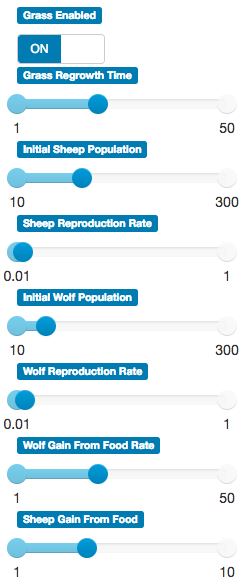
\includegraphics[width=4cm]{case_1_vars}
		\centering
		\color{blue}
		\caption{Cas 1 - Valors de les variables.}\label{visina8}
	\end{figure}

	Les gràfiques obtingudes per a una simulació en concret de les situacions anteriors són les següents:

	\begin{figure}[H]
		\begin{changemargin}{-1cm}{0.5cm}
			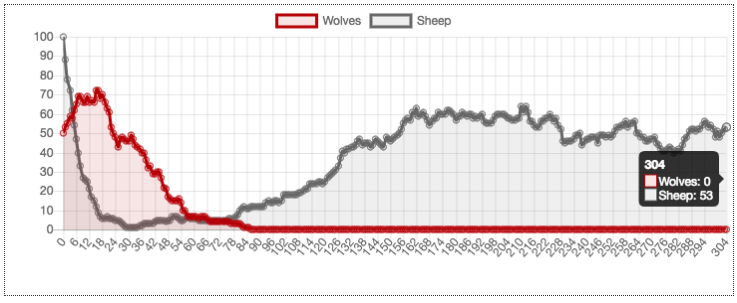
\includegraphics[width=14cm]{case_1_graph_sheeps}
			\centering
			\color{blue}
			\caption{Cas 1 - Situació 1. Gràfic de l'evolució de les ovelles i els llops.}\label{visina8}
		\end{changemargin}
	\end{figure}

	\begin{figure}[H]
		\begin{changemargin}{-1cm}{0.5cm}
			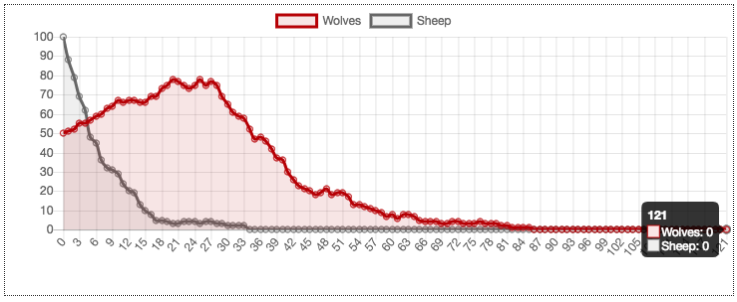
\includegraphics[width=14cm]{case_1_graph_grass}
			\centering
			\color{blue}
			\caption{Cas 1 - Situació 2. Gràfic de l'evolució de les ovelles i els llops.}\label{visina8}
		\end{changemargin}
	\end{figure}

	\subsection*{Cas 2 (sense modificar del codi):}
	Jugant amb els paràmetres he pogut comprovar que només modificant la tasa de reproducció de les ovelles, s'aconsegueix arribar a una situació bastant més estable. \\

	De totes maneres, les fluctuacions del nombre d'ovelles i llops són evidents i bastant brusques. Cal dir, també, que en alguna de les múltiples execucions de la simulació d'aquest cas, he observat que s'ha arribat a la situació d'aniquilar totalment les ovelles. \\

	{\fontfamily{pcr}\selectfont\small
	\begin{tabular}{l | r}
		\multicolumn{2}{c}{Cas 2}  \\ \hline
		Variable & Valor \\ \hline
		Grass enabled &  True  \\
		Grass Regrowth Time &  20  \\
		Initial Sheep Population &  100  \\
		Sheep Reproduction Rate &  \textbf{0.23}  \\
		Initial Wolf Population &  50  \\
		Wolf Reproduction Rate &  0.05  \\
		Wolf Gain From Food Rate &  20  \\
		Sheep Gain From Food &  4  \\
	\end{tabular}
	} \\

	\begin{figure}[H]
		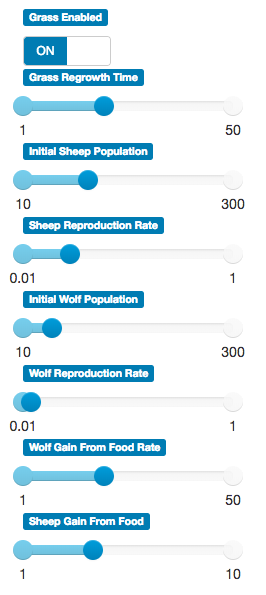
\includegraphics[width=4cm]{case_2_vars}
		\centering
		\color{blue}
		\caption{Cas 2 - Valors de les variables.}\label{visina8}
	\end{figure}

	\begin{figure}[H]
		\begin{changemargin}{-1cm}{0.5cm}
			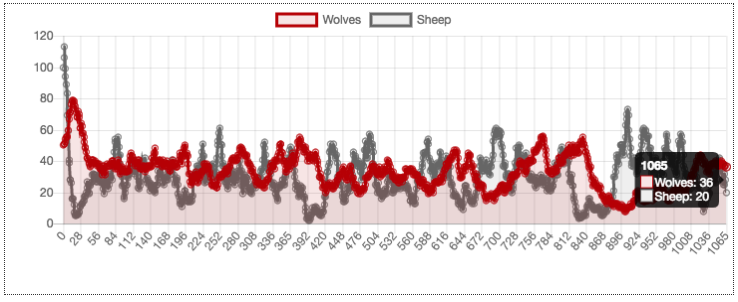
\includegraphics[width=14cm]{case_2_graph}
			\centering
			\color{blue}
			\caption{Cas 2 - Gràfic de l'evolució de les ovelles i els llops.}\label{visina8}
		\end{changemargin}
	\end{figure}

	\subsection*{Cas 3 (sense modificar del codi):}
	Llavors, he modificat pràcticament el valor de totes les variables, buscant que pogués mantenir-se estable, dintre d'uns marges de variabilitat. I he trobat que la següent combinació dóna uns resultats bastant interessants: \\

	{\fontfamily{pcr}\selectfont\small
	\begin{tabular}{l | r}
		\multicolumn{2}{c}{Cas 3}  \\ \hline
		Variable & Valor \\ \hline
		Grass enabled & True \\
		Grass Regrowth Time & \textbf{31} \\
		Initial Sheep Population & 100 \\
		Sheep Reproduction Rate & \textbf{0.09} \\
		Initial Wolf Population & \textbf{18} \\
		Wolf Reproduction Rate & \textbf{0.01} \\
		Wolf Gain From Food Rate & 20 \\
		Sheep Gain From Food & \textbf{10}\\
	\end{tabular}
	} \\

	\begin{figure}[H]
		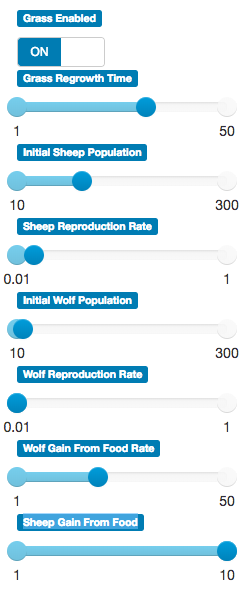
\includegraphics[width=4cm]{case_10_vars}
		\centering
		\color{blue}
		\caption{Cas 3 - Valors de les variables.}\label{visina8}
	\end{figure}

	Al gràfic, es pot observar que el nombre d'ovelles i llops fluctuen, però menys brúscament que al cas anterior. Això, és degut, en part, a que s'ha reduït la població inicial de llops i la seva probabilitat de repoducció. També, s'ha incrementat el guany de menjar de les ovelles i la seva probabilitat de reproducció. A més, per tal de compensar el guany de menjar de les ovelles, s'ha incrementat el temps de l'herba de tornar a estar al nivell màxim per a ser menjada. \\

	El resultat és que les fluctuacions són més suaus i permeten mantenir l'ecosistema més estable.

	\begin{figure}[H]
		\begin{changemargin}{-1cm}{0.5cm}
			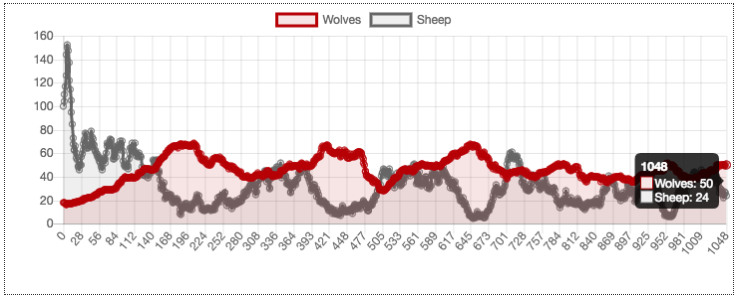
\includegraphics[width=14cm]{case_10_graph_2}
			\centering
			\color{blue}
			\caption{Cas 3 - Gràfic de l'evolució de les ovelles i els llops.}\label{visina8}
		\end{changemargin}
	\end{figure}

	\subsection*{Modificacions del codi:}
	Ara, he aplicat les modificacions que se'ns demana a l'enunciat: afegit la variable edat per als agents Sheep i Wolf. És a dir, a partir d'ara, les ovelles i els llops només es podran reproduir si tenen més d'un any de vida i, al cap de 20 anys, moriran. \\

	He considerat, tal i com es recomanava a l'enunciat, que una iteració equival a un mes de vida. \\

	Els canvis aplicats al codi són els següents: \\

	\begin{figure}[H]
		\begin{changemargin}{-1cm}{0.5cm}
			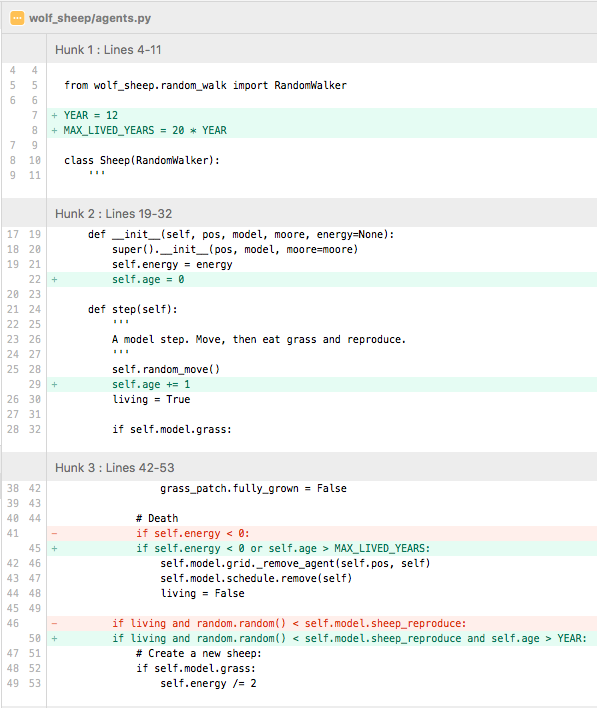
\includegraphics[width=14cm]{code/agents_1}
			\centering
			\color{blue}
			\caption{Modificacions al codi. Arxiu agents.py}\label{visina8}
		\end{changemargin}
	\end{figure}

	\begin{figure}[H]
		\begin{changemargin}{-1cm}{0.5cm}
			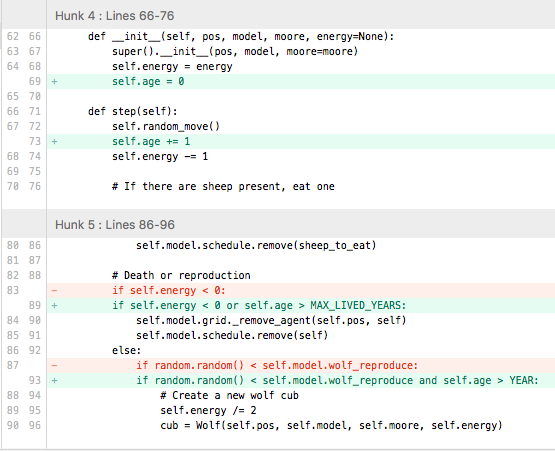
\includegraphics[width=14cm]{code/agents_2}
			\centering
			\color{blue}
			\caption{Modificacions al codi. Arxiu agents.py}\label{visina8}
		\end{changemargin}
	\end{figure}

	\begin{figure}[H]
		\begin{changemargin}{-1cm}{0.5cm}
			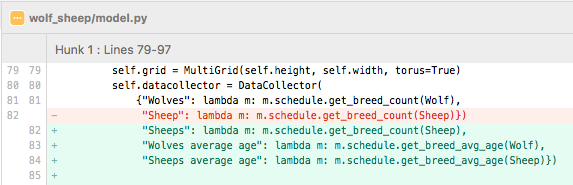
\includegraphics[width=14cm]{code/model}
			\centering
			\color{blue}
			\caption{Modificacions al codi. Arxiu model.py}\label{visina8}
		\end{changemargin}
	\end{figure}

	\begin{figure}[H]
		\begin{changemargin}{-1cm}{0.5cm}
			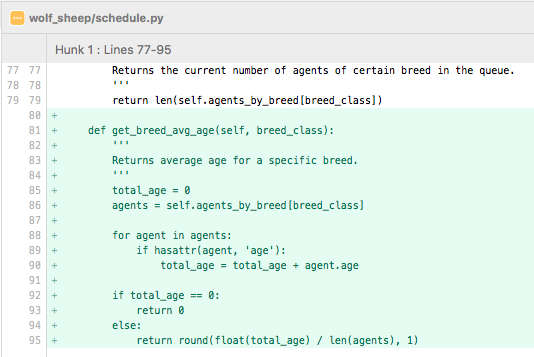
\includegraphics[width=14cm]{code/schedule}
			\centering
			\color{blue}
			\caption{Modificacions al codi. Arxiu schedule.py}\label{visina8}
		\end{changemargin}
	\end{figure}

	\begin{figure}[H]
		\begin{changemargin}{-1cm}{0.5cm}
			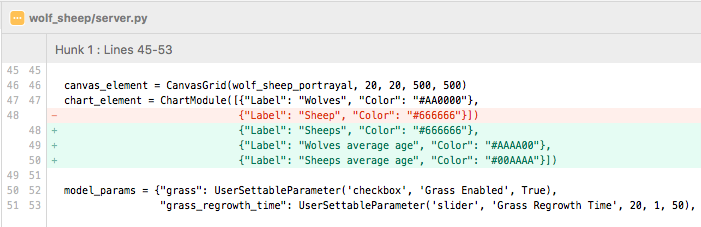
\includegraphics[width=14cm]{code/server}
			\centering
			\color{blue}
			\caption{Modificacions al codi. Arxiu server.py}\label{visina8}
		\end{changemargin}
	\end{figure}

	\subsection*{Cas 1 (amb el codi modificat):}

	Si es torna a executar els casos anteriors, es pot observar que, per als paràmetres del primer cas, es segueix obtenint els dos tipus de situacions: o bé, els llops es mengen les ovelles i després moren de fam (falta d'energia), o bé, els llops es moren i les ovelles aconsegueixen sobreviure obtenint una població mitjana al voltant dels 50 exemplars. \\

	També es pot veure, al gràfic de la situació 1, que la mitjana de l'edat de les ovelles es troba als voltants dels 40 mesos (3 anys i 4 mesos). Cal dir, que la causa principal de mort de les ovelles és degut a la falta de menjar i que molt poques ovelles moren com a conseqüència d'haver arribat als 20 anys de vida (a partir de la iteració 240). Els llops també moren per falta de menjar. \\

	Per tal de visualitzar aquesta informació he afegit {\fontfamily{pcr}\selectfont\small print} al codi (no es mostra a les imatges anteriors de les modificacions). \\

	En el gràfic de la situació 2, les ovelles es moren perquè els llops se les mengen i els llops es moren tots de fam (no arriben a la iteració 240). \\

	\begin{figure}[H]
		\begin{changemargin}{-1cm}{0.5cm}
			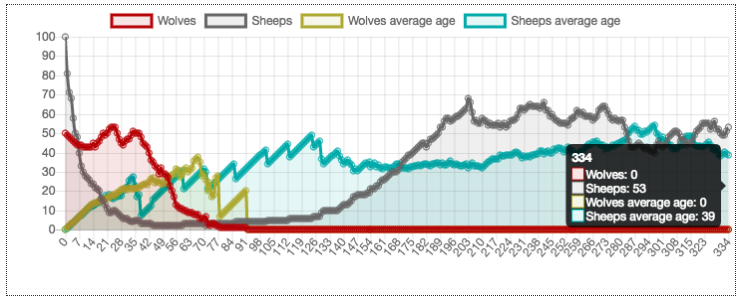
\includegraphics[width=14cm]{mod_case_1_graph_sheeps}
			\centering
			\color{blue}
			\caption{Cas 1 - Situació 1. Gràfic de l'evolució de les ovelles i els llops.}\label{visina8}
		\end{changemargin}
	\end{figure}

	\begin{figure}[H]
		\begin{changemargin}{-1cm}{0.5cm}
			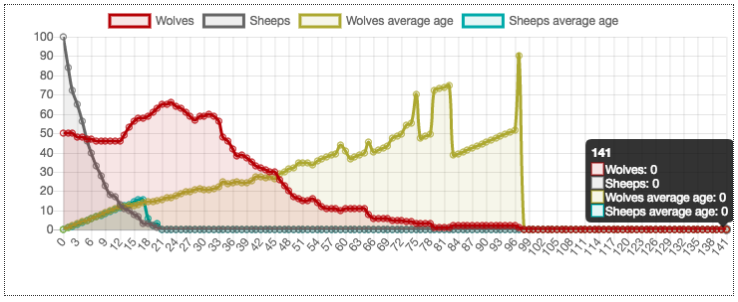
\includegraphics[width=14cm]{mod_case_1_graph_grass}
			\centering
			\color{blue}
			\caption{Cas 1 - Situació 2. Gràfic de l'evolució de les ovelles i els llops.}\label{visina8}
		\end{changemargin}
	\end{figure}

	\subsection*{Cas 2 (amb el codi modificat):}

	En aquest cas, es veu com les ovelles es mantenen en una mitjana d'edat al voltant dels 10 mesos, mentre que els llops tenen una mitjana d'edat molt més alta (al voltant dels 30 mesos, és a dir, 2 anys i 6 mesos). De totes formes i, tal i com he comentat al cas anterior, els agents (ovelles o llops) que es moren per arribar al seu màxim d'edat és molt reduït, la gran majoria moren de fam. \\

	\begin{figure}[H]
		\begin{changemargin}{-1cm}{0.5cm}
			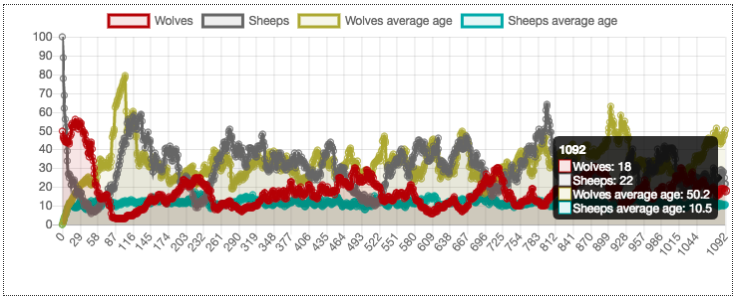
\includegraphics[width=14cm]{mod_case_2_graph}
			\centering
			\color{blue}
			\caption{Cas 2 - Gràfic de l'evolució de les ovelles i els llops.}\label{visina8}
		\end{changemargin}
	\end{figure}

	\subsection*{Cas 3 (amb el codi modificat):}

	En aquest cas, s'observa que la mitjana d'edat dels llops ha augmentat considerablement (al voltant dels 100 mesos, és a dir, 8 anys i 4 mesos) i la mitjana de d'edat de les ovelles es manté al voltant dels 20 mesos (1 any i 8 mesos). \\

	Tot i això, es segueix mantenint la dinàmica que els agents es moren de fam i no de vells. \\

	\begin{figure}[H]
		\begin{changemargin}{-1cm}{0.5cm}
			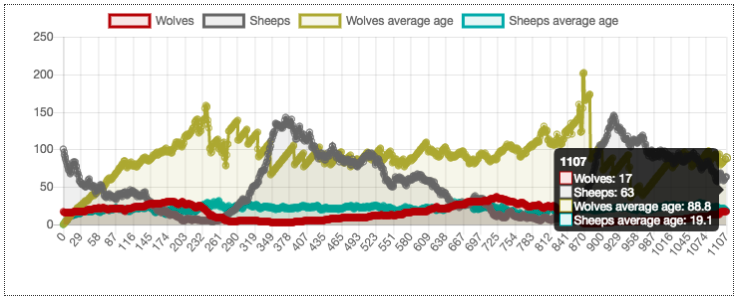
\includegraphics[width=14cm]{mod_case_10_graph_2}
			\centering
			\color{blue}
			\caption{Cas 3 - Gràfic de l'evolució de les ovelles i els llops.}\label{visina8}
		\end{changemargin}
	\end{figure}

	\subsection*{Cas 4 (amb el codi modificat):}

	Per tal d'intentar observar els efectes d'haver afegit la variable edat, he modificat tots els paràmetres deixant-los al mínim, excepte el del guany del menjar per a les ovelles, que l'he col·locat al màxim. D'aquesta manera, he reduït, expressament, al màxim la vida i la supervivència dels llops, i he augmentat la supervivència, però no reproducció de les ovelles. Això, hauria de permetre que un agent Sheep tingués menjar suficient i sempre disponible per a la seva supervivència i, així, només hauria de morir de vellesa. \\

	Cal remarcar que m'he centrat en el cas de mantenir vives les ovelles i no els llops, ja que és molt més senzill d'aconseguir i el sistema resultant és molt més simple. Només cal centrar-se en 2 agents: Sheep i GrassPatch, ja que l'agent Wolf queda eliminat ben al principi. \\

	En executar la simulació, a la figura \ref{fig:cas4-zoom274}, sí que es veu que a la iteració 240 hi ha una davallada de 10 ovelles (són les ovelles inicials de partida), però a la llarga se'n reprodueixen més que no pas moren d'envelliment (a la primera fase pràcticament cap mor de fam). Finalment, tal i com es pot observar a la figura \ref{fig:cas4-complete}, quan s'estabilitza la situació, moltes de les ovelles tornen a morir per falta de menjar. De totes maneres, cal dir, que, un cop estabilitzat, sí que hem aconseguit un ratio més elevat de morts per envelliment (aproximadament una tercera part). Això queda reflectit a la mitjana d'edat de les ovelles, que ara es troba al voltant dels 95 mesos (7 anys i 11 mesos).\\

	També, a la figura \ref{fig:cas4-zoom29}, es pot observar com durant els primers 29 mesos, la mitjana d'edat augmenta linealment ja que no hi ha cap ovella que es mori menjada pels llops (en aquesta simulació, els llops moren sense haver aconseguit menjar cap ovella) i perquè tampoc aconsegueixen reproduir-se (recordar que tenim la condició de que no es poden reproduir si no tenen 12 mesos com a mínim de vida). \\

	{\fontfamily{pcr}\selectfont\small
	\begin{tabular}{l | r}
		\multicolumn{2}{c}{Cas 4}  \\ \hline
		Variable & Valor \\ \hline
		Grass enabled &  True  \\
		Grass Regrowth Time &  \textbf{1}  \\
		Initial Sheep Population &  \textbf{10}  \\
		Sheep Reproduction Rate &  \textbf{0.01}  \\
		Initial Wolf Population &  \textbf{10}  \\
		Wolf Reproduction Rate &  \textbf{0.01}  \\
		Wolf Gain From Food Rate &  \textbf{1}  \\
		Sheep Gain From Food &  \textbf{10}  \\
	\end{tabular}
	} \\

	\begin{figure}[H]
		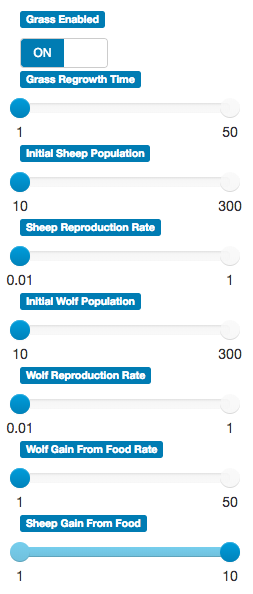
\includegraphics[width=4cm]{mod_case_12_vars}
		\centering
		\color{blue}
		\caption{Cas 4 - Valors de les variables.}\label{visina8}
	\end{figure}

	\begin{figure}[H]
		\begin{changemargin}{-1cm}{0.5cm}
			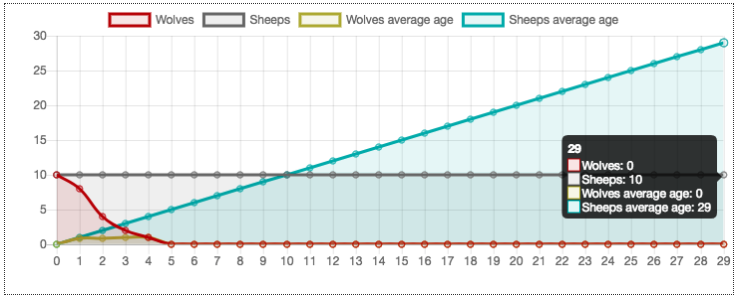
\includegraphics[width=14cm]{mod_case_12_graph_1}
			\centering
			\color{blue}
			\caption{Cas 4 - Gràfic de l'evolució de les ovelles i els llops. Zoom per a les 29 primeres iteracions.}\label{visina8}
  			\label{fig:cas4-zoom29}
		\end{changemargin}
	\end{figure}

	\begin{figure}[H]
		\begin{changemargin}{-1cm}{0.5cm}
			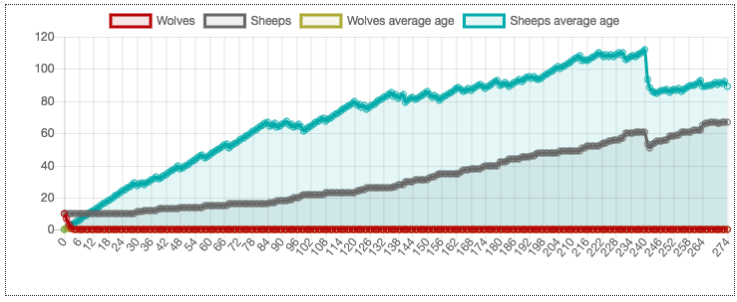
\includegraphics[width=14cm]{mod_case_12_graph_2}
			\centering
			\color{blue}
			\caption{Cas 4 - Gràfic de l'evolució de les ovelles i els llops. Zoom per a les 274 primeres iteracions.}\label{visina8}
  			\label{fig:cas4-zoom274}
		\end{changemargin}
	\end{figure}

	\begin{figure}[H]
		\begin{changemargin}{-1cm}{0.5cm}
			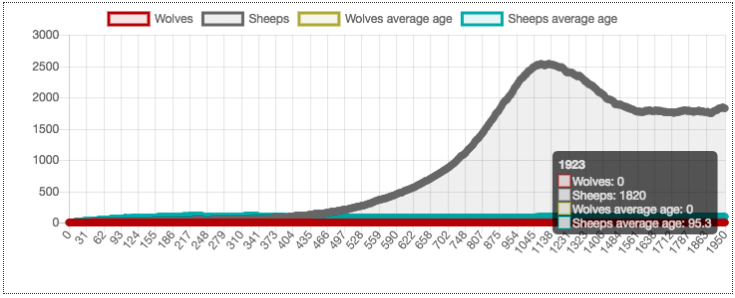
\includegraphics[width=14cm]{mod_case_12_graph_3}
			\centering
			\color{blue}
			\caption{Cas 4 - Gràfic de l'evolució de les ovelles i els llops. Simulació completa.}\label{visina8}
  			\label{fig:cas4-complete}
		\end{changemargin}
	\end{figure}
}

\section{Exercici 3}
En un sistema multi-agent on els agents sheep i Wolf poden comunicar-se entre ells,
penseu 2 tipus d'accions podrien realitzar per fer més realista el sistema, quin
protocol FIPA utilitzarien i que informació es passarien. \\

{\color{blue}
	Es podria pensar en un sistema de comunicació centralitzada a nivell de tipus d'agent (o Sheep o Wolf, suposem que GrassPatch no té capacitat de reaccionar als estimuls externs ni intel·ligència), els agents d'un tipus en particular es podrien comunicar a través d'una pissarra informant de la seva posició, posició dels altres agents al seu voltant i comunicació d'on són les possibles preses o depredadors i, en el cas de les ovelles, els trossos d'herba per a poder alimentar-se. \\

	Els agents d'un tipus concret podrien accedir a aquesta informació i utilitzar-la per prendre decisions per fer més eficient la seva distribució a la quadrícula. A més, disposar d’informació de varis agents (en alguns casos redundant) milloraria la robustesa i riquesa de coneixement del sistema a l’hora de prendre decisions. Així, podríem definir dos tipus de comunicacions:


	\begin{itemize}
		\item {Una ovella es vol comunicar amb altres ovelles per saber si es pot menjar un tros d'herba. Utilitzaria el FIPA-Request per a perguntar si hi ha alguna altra ovella a la mateixa casella que estigui més necessitada que ella (tingui menys energia i no sigui vella).

		En aquest cas, fins i tot, es podria afegir algun tipus de lògica fent que si una altra ovella no es troba a la mateixa casella però molt aprop i realment està molt més necessitada que l'actual, li indiqui la coordenada a la qual s'ha de moure i li cedeixi l'herba a l'espera que en els següents torns se la pugui menjar.}

		\item {Un llop es vol comunicar amb altres llops per saber si pot menjar-se una ovella. Utilitzaria el FIPA-Request per a perguntar si hi ha algun altre llop a la mateixa casella que estigui més necessitat que ell (tingui menys energia i no sigui vell). 

		En aquest cas, no tindria massa sentit que un llop cedís una ovella a algun altre llop que es trobés aprop de la casella i més necessitat, ja que les ovelles van canviant de posició i, a no ser que s'afegís algun tipus d'intel·ligència als llops per a permetre seguir-les, es podria perdre el seu rastre en els torns següents.}
	\end{itemize}
}

\end{document}